% !TEX program = xelatex
\documentclass[11pt]{ctexart}

\usepackage[a4paper,margin=2.4cm]{geometry}
\usepackage{graphicx}
\usepackage{amsmath}
\usepackage{booktabs}
\usepackage{tikz}
\usetikzlibrary{arrows.meta,positioning}
\usepackage{xcolor}
\usepackage[most]{tcolorbox}
\usepackage{listings}
\usepackage{float}
\usepackage[colorlinks=true,linkcolor=blue!60!black,urlcolor=blue!60!black]{hyperref}

\definecolor{plainC}{RGB}{235,244,255}
\definecolor{toyC}{RGB}{236,250,236}
\definecolor{codegray}{RGB}{246,246,246}

\newtcolorbox{whybox}[1][]{breakable,enhanced,colback=plainC,colframe=blue!45!black,
  title={\textbf{这一站在干什么} #1},fonttitle=\small,left=2mm,right=2mm,top=1mm,bottom=1mm}
\newtcolorbox{toybox}[1][]{breakable,enhanced,colback=toyC,colframe=green!40!black,
  title={\textbf{玩具小区实跑} #1},fonttitle=\small,left=2mm,right=2mm,top=1mm,bottom=1mm}

\lstset{language=Python, basicstyle=\ttfamily\footnotesize,
  numbers=left, numberstyle=\tiny\color{gray}, numbersep=6pt,
  backgroundcolor=\color{codegray}, frame=single, framerule=0.3pt,
  rulecolor=\color{gray!50}, breaklines=true, columns=fullflexible,
  keepspaces=true, showstringspaces=false,
  keywordstyle=\color{blue!55!black}\bfseries,
  commentstyle=\color{green!40!black}, stringstyle=\color{orange!60!black}}

\setlength{\parskip}{0.45em}

\title{\textbf{代码走读：RandLA-Net 的标签是怎么变成一栋栋楼的}\\[0.3em]
\Large \texttt{instance\_segmentation\_v2.py} 九站流水线 · 玩具小区实跑版}
\author{Columbus LiDAR $\to$ LOD2 管线 · 02\_03 汇报准备材料（第二册）}
\date{2026 年 8 月 30 日}

\begin{document}
\maketitle

\section*{这本讲义怎么用}

上一册从概念讲起，你觉得隔了一层。这一册换个路子：\textbf{直接顺着源代码讲}。
生成实例数据的其实就一个脚本
——\texttt{02\_03\_instance\_seg/instance\_segmentation\_v2.py}，一共 336 行。
我把它切成九站，每一站给你三样东西：

\begin{enumerate}
\item \textbf{一段真实源码}。带原文件行号，想细看可以照着行号翻源文件。
      片段里偶尔用 \texttt{...} 跳过几行不重要的，跳过之后行号会有点对不上，
      找代码时认准每站标题里写的行号范围就行。
\item \textbf{一个蓝框}，说这段代码是来干什么活的。不抠语法，只讲事。
\item \textbf{一个绿框加一张图}，让你亲眼看效果。我搭了一个 25 米 $\times$ 18 米的
      玩具小区，照着源码把算法重写了一遍（操作和参数一模一样，只简化了坐标原点、
      网格留边这类无关紧要的细节），一站一站跑给你看。
      每张图都是程序真跑出来的，不是画的示意图。
\end{enumerate}

生成玩具场景、逐站出图的脚本叫 \texttt{toy\_pipeline.py}，就放在本文档同目录下，
运行 \texttt{python3 toy\_pipeline.py} 随时能重跑。

\subsection*{玩具小区里都有什么}

场景是精心安排过的：每个成员都对应真实数据里的一类情况，
专门用来触发流水线的某一个环节。

\begin{center}
\small
\begin{tabular}{llp{7.6cm}}
\toprule
成员 & 尺寸 / 高度 & 安排它进来的用意 \\
\midrule
住宅 A（人字顶） & $10\times8$ m，屋檐 4.6 / 屋脊 6.0 m & 主角。屋顶挖了个 $1.5\times1.5$ m 的洞，模拟树冠遮挡 \\
平顶房 B & $9\times7$ m，4.0 m & 和 A 之间隔一条 2 m 宽的侧院 \\
树枝桥接点 & $2\times1.5$ m 一小条，2.8 m & 被错标成``建筑''的树枝，正好把 A 和 B 连在一起，等分水岭来拆 \\
门廊碎片 & $3\times2.5$ m（7.5 m\textsuperscript{2}），3.2 m & 离 A 只有 1 m 的小碎块，等着被``碎片吸收''收编 \\
棚屋 C & $5\times4.6$ m（23 m\textsuperscript{2}），3.0 m & 一栋独立小房，用来验证不该拆的不拆、不该吸的不吸 \\
错标停车场 & $6\times5$ m（30 m\textsuperscript{2}），0.15 m & 贴着地的错标。这个脚本拿它没办法，得靠 Gate A 算离地高度 \\
零星错点 & 5 个孤点，一格一个 & 想搭``一点桥''，被``每格至少 2 点''的规则拦住（点本身的下场见第 9 站） \\
杂物团 & $2\times1.5$ m（3 m\textsuperscript{2}），1.5 m & 孤零零的小渣，整块过不了``20 m\textsuperscript{2} 起步''这道线 \\
屋檐稀疏点 & A 左侧 0.5 m 窄条，一格约 1 点 & 先被占据规则放下，最后靠``孤儿点回挂''捡回来 \\
\bottomrule
\end{tabular}
\end{center}

场景里另外撒了一层\textbf{地面点}（类别 2），留给最后一站建 DTM 用。
图~\ref{fig:scene} 是全家福。看图时记住一件事：
\textbf{图上的颜色是我们站在上帝视角标的，程序看不到}。
程序拿到手的，只是一堆标签都写着``建筑''的裸点。
谁是楼、谁是树枝、谁是停车场，要靠下面九站自己分出来。

\begin{figure}[H]
\centering
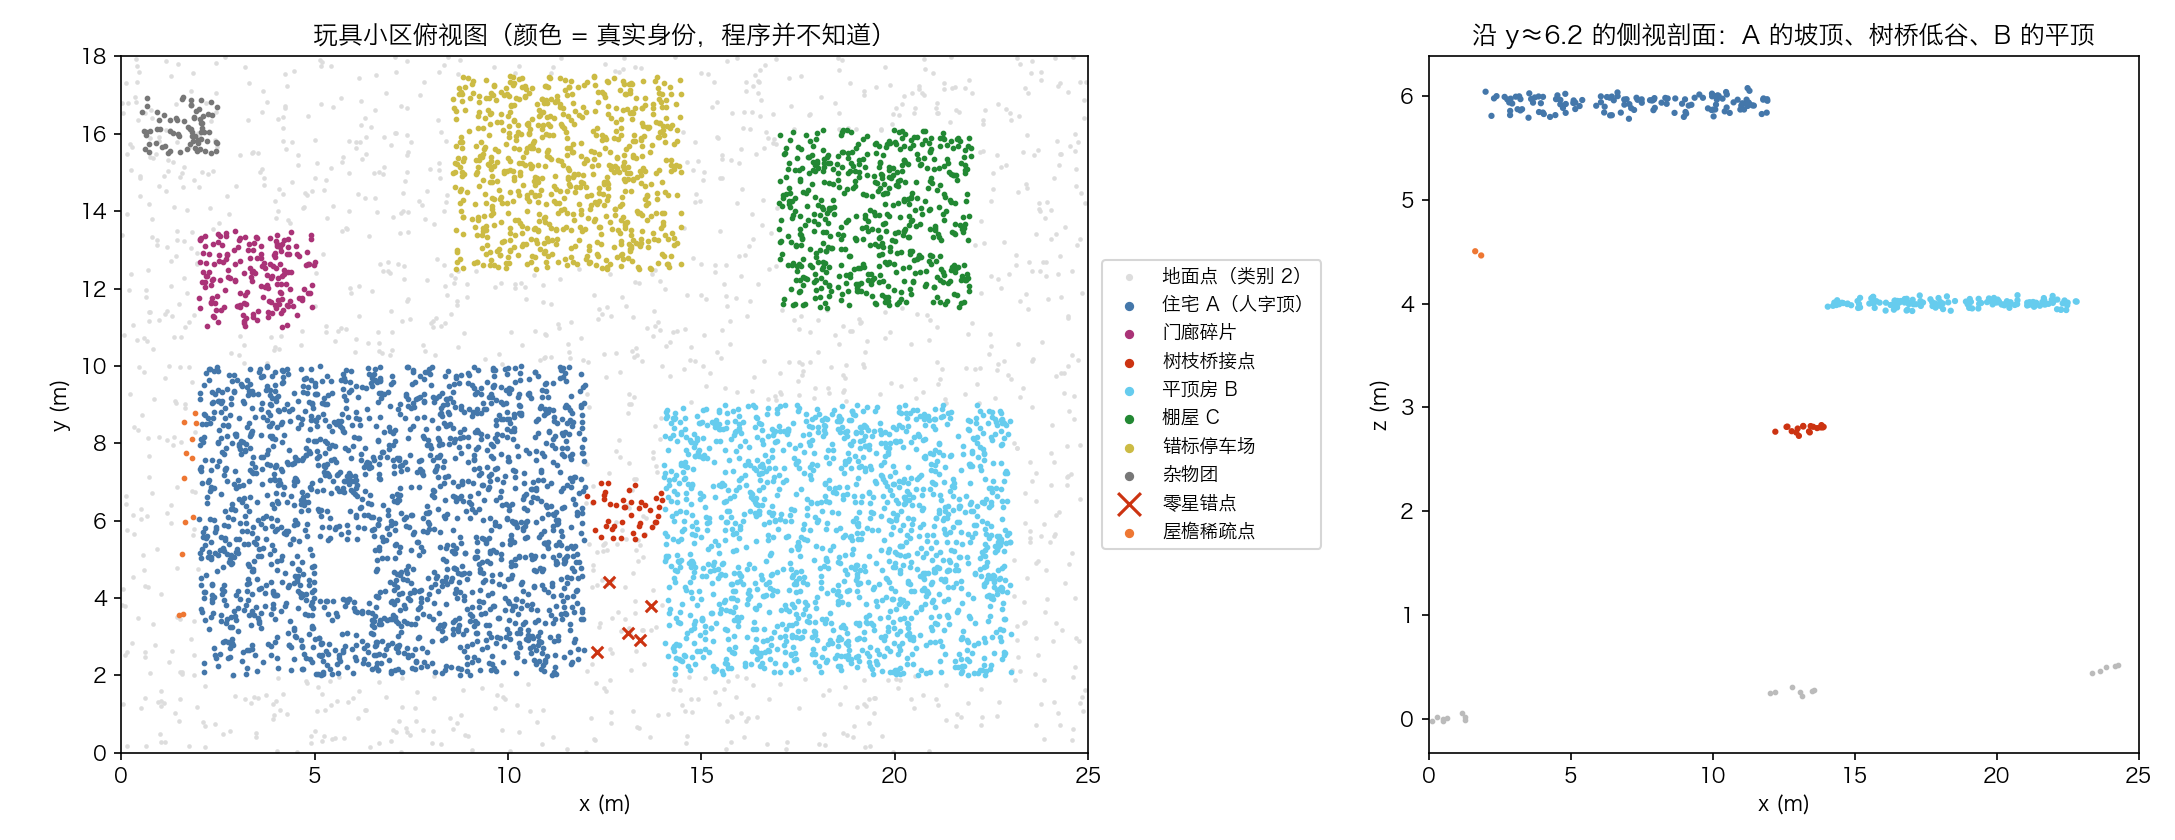
\includegraphics[width=\textwidth]{figs/toy_f1_scene.png}
\caption{玩具小区。左：俯视图，灰色是地面点。右：沿 $y\approx6.2$ 切一刀的侧视剖面，
能看到 A 的坡屋顶（约 6 m）、树桥的低谷（2.8 m）、B 的平顶（4.0 m）。}
\label{fig:scene}
\end{figure}

\section{全景：九站流水线}

\begin{center}
\begin{tikzpicture}[node distance=0.34cm, every node/.style={font=\scriptsize}]
\tikzstyle{st}=[draw, rounded corners, minimum height=0.72cm, text width=1.72cm, align=center, fill=blue!8]
\node[st] (s1) {1 读数据\\挑建筑点};
\node[st, right=of s1] (s2) {2 英尺\\换米};
\node[st, right=of s2] (s3) {3 栅格化\\+占据};
\node[st, right=of s3] (s4) {4 连通域};
\node[st, right=of s4] (s5) {5 逐块\\补洞};
\node[st, right=of s5] (s6) {6 腐蚀\\取核};
\node[st, right=of s6] (s7) {7 分水岭\\拆粘连};
\foreach \a/\b in {s1/s2,s2/s3,s3/s4,s4/s5,s5/s6,s6/s7}
  \draw[-{Stealth}] (\a) -- (\b);
\node[st, below=0.5cm of s7] (s8) {8 碎片\\吸收};
\node[st, left=of s8] (s9) {9 丢渣·发号\\·捡孤儿};
\node[st, left=of s9, fill=green!12] (out) {写出\\instance\_id};
\draw[-{Stealth}] (s7) -- (s8);
\draw[-{Stealth}] (s8) -- (s9);
\draw[-{Stealth}] (s9) -- (out);
\end{tikzpicture}
\end{center}

整个脚本一句话就能说明白：\textbf{把 863 万个三维点压成一张 0.5 米一格的二维图，
在图上分块、拆开粘连、收拾碎片，最后把每个格子分到的楼编号，
写回落在这个格子里的每一个点}。下面一站一站讲。
行号都指 \texttt{instance\_segmentation\_v2.py} 原文件。

\section{第 1 站（83--99 行）：读 19 块瓦片，只留``建筑''点}

\begin{lstlisting}[firstnumber=86]
    for i, t in enumerate(tiles):
        las = laspy.read(t)
        ...
        m = np.asarray(las.classification) == BUILDING_CLASS   # 6
        xs.append(np.asarray(las.x)[m])
        ys.append(np.asarray(las.y)[m])
        zs.append(np.asarray(las.z)[m])
\end{lstlisting}

\begin{whybox}
RandLA-Net 交出来的是 19 个点云文件，每个点带一个类别码：2 是地面、5 是植被、
6 是建筑、1 是其他。这一站就做两件事：把 19 个文件的点拼到一起；
再拿 \texttt{classification == 6} 筛一遍，只留下标签写着``建筑''的点。
后面所有步骤，处理的都只是这批点。
不过``标签写着建筑''不等于``真是建筑''——筛出来的点里混着错标的树枝、
停车场、电线，收拾它们正是后面各站的活儿。
\end{whybox}

\begin{toybox}
玩具小区里标签为``建筑''的点一共 \textbf{4{,}964 个}，
也就是图~\ref{fig:scene} 里除去灰色地面点之外的全部，树桥、停车场这些冒牌货都在内。
真实数据在这一步筛出约 863 万个点。
\end{toybox}

\section{第 2 站（101 行）：英尺换成米}

\begin{lstlisting}[firstnumber=101]
    xm = x_ft * FT_TO_M; ym = y_ft * FT_TO_M; zm = z_ft * FT_TO_M
\end{lstlisting}

\begin{whybox}
原始数据用的是美制测量英尺（美国官方测绘数据的老习惯），乘上 0.3048\ldots{}
这个常数，全部换成米。别看只有一行，它配得上单独一站：
后面所有阈值——0.5 米的格子、1.5 米的腐蚀、3 米的吸收距离——全是按米定的。
这里单位一错，后面全盘皆错。
\end{whybox}

\section{第 3 站（103--116 行）：栅格化——数格子、记最高点}

\begin{lstlisting}[firstnumber=104]
    x0, y0 = xm.min(), ym.min()
    ix = ((xm - x0) / CELL).astype(np.int32)   # CELL = 0.5 m
    iy = ((ym - y0) / CELL).astype(np.int32)
    ...
    cnt = np.zeros((ny, nx), np.uint16)
    np.add.at(cnt, (iy, ix), 1)            # 每格数一数落了几个点
    occ = cnt >= MIN_PTS_CELL              # >=2 点才算"被建筑占据"
    zg = np.full((ny, nx), -1e9, np.float32)
    np.maximum.at(zg, (iy, ix), zm.astype(np.float32))  # 每格记最高点
\end{lstlisting}

\begin{whybox}
想象在小区上空铺一张 0.5 米一格的方格纸。每个点拿自己的坐标除以 0.5、取整，
就知道自己落在第几行第几列。落格之后，程序做出三张``图''：
\begin{itemize}
\item \texttt{cnt}，\textbf{计数图}：每格落了几个点。\texttt{np.add.at}
      干的就是``逐点跑到对应格子上画正字''这件事。
\item \texttt{occ}，\textbf{占据图}：数够 2 个点的格子，才算``这里有建筑''。
      为什么要够 2 个？因为孤零零一个错点不该让一个格子算数——不设这道门槛，
      零星错点就能在两栋楼之间连出一条``一点桥''。
\item \texttt{zg}，\textbf{高度图}：每格记下格内最高点的高程。现在用不上，
      第 7 站分水岭全指着它。
\end{itemize}
到这里，863 万个点的难题就变成了一张几千乘几千的二维图。
\end{whybox}

\begin{toybox}
看图~\ref{fig:raster}。左边是放大镜，格子上的数字就是 \texttt{cnt} 的值：
零星错点占的格子都只数到 \textcolor{red!70!black}{\textbf{1}}（红字），
不够 2，这格不算数。右边是整张占据图：\textbf{809 个}格子被占据；
\textbf{34 个}只有 1 个点的格子（浅红色）被放下，5 个零星错点全在里面
——``一点桥''从源头就没搭起来。再留意一下：A 屋顶上的洞、A 和 B 之间的侧院缝，
这时候都还原样留着。
\end{toybox}

\begin{figure}[H]
\centering
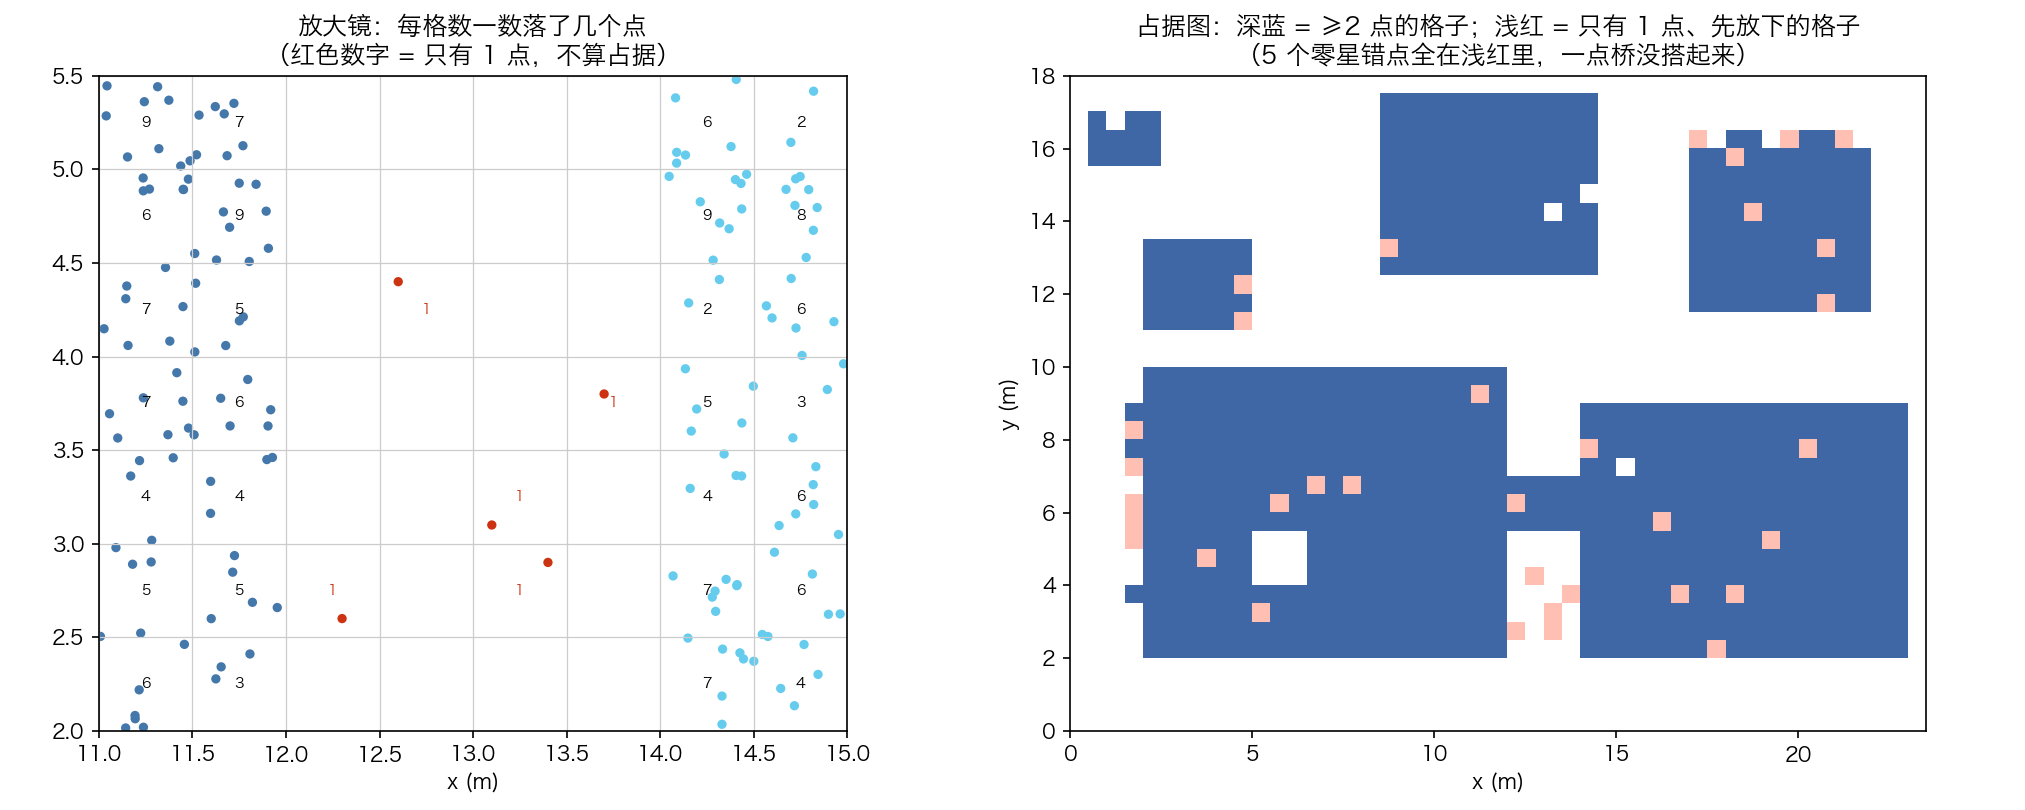
\includegraphics[width=\textwidth]{figs/toy_f2_raster.png}
\caption{第 3 站前后：左边是点云和每格的计数，右边是得到的占据图。}
\label{fig:raster}
\end{figure}

\section{第 4 站（119--121 行）：连通域——挨着的格子算一块}

\begin{lstlisting}[firstnumber=119]
    s8 = np.ones((3, 3), bool)                 # "邻居"= 周围 8 个格子
    comps0, nc0 = ndimage.label(occ, structure=s8)
\end{lstlisting}

\begin{whybox}
\texttt{ndimage.label} 是图像处理里的基础工具：在黑白的占据图上，
把互相挨着的格子（上下左右加四个斜角，一共 8 个方向）归成一``块''，
一块发一个临时编号。这就是单体化的第一刀。大部分块这时已经正好是一栋楼了；
麻烦在于，\textbf{只要两栋楼之间有东西连着，哪怕是几个错点，它们就会被算成同一块}。
\end{whybox}

\begin{toybox}
玩具小区标出 \textbf{5 个块}（图~\ref{fig:comps}）：门廊、棚屋 C、停车场、
杂物团各自成块；而 \textbf{A、树桥、B 被连成了一整个大块}，图上是同一种蓝色。
真实数据里``树把两栋楼粘到一起''就是这个样子。这时候程序还不知道大块有毛病
——发现它、拆开它，是第 6、7 站的事。
\end{toybox}

\begin{figure}[H]
\centering
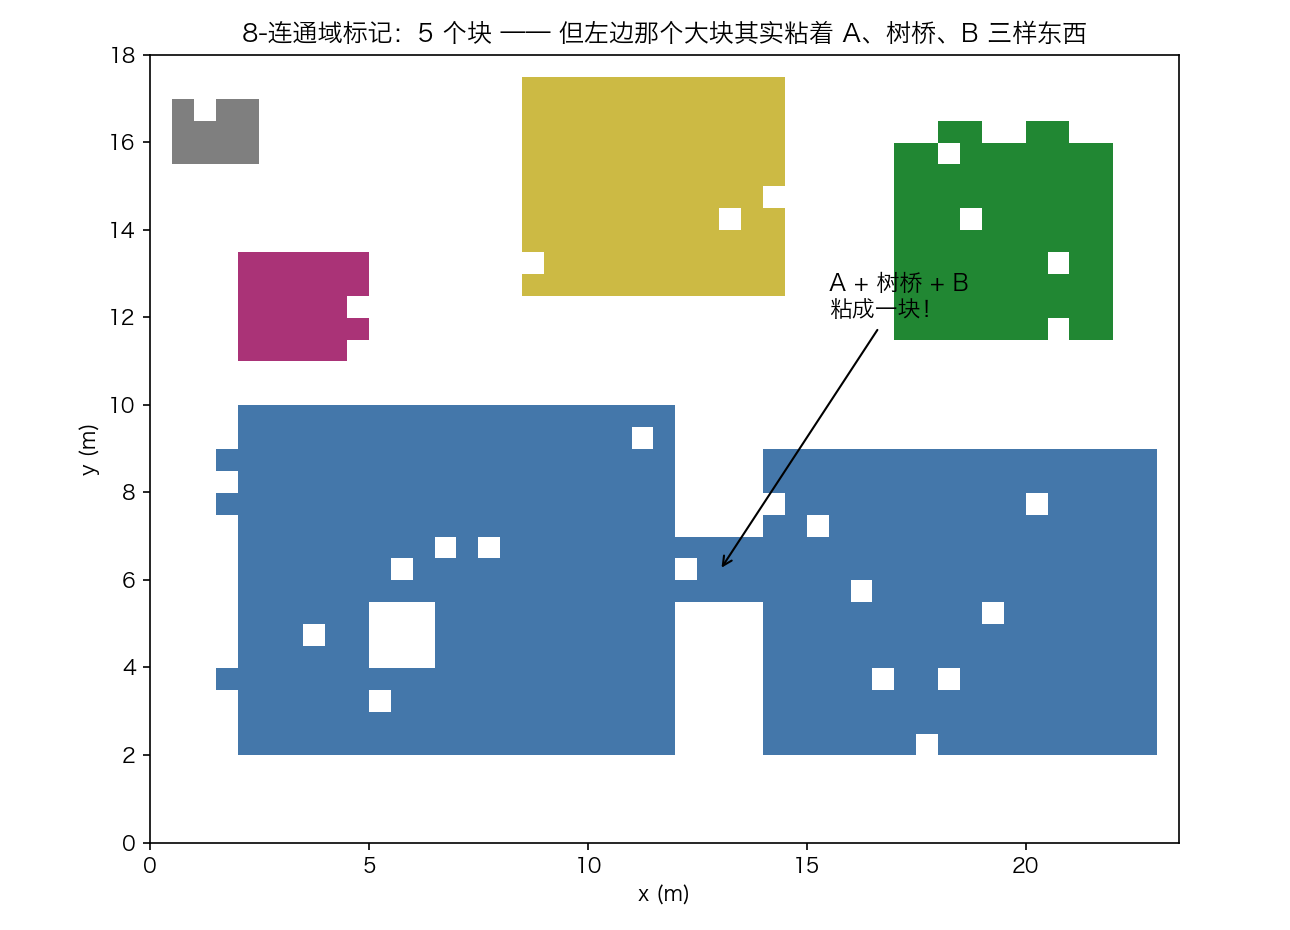
\includegraphics[width=0.72\textwidth]{figs/toy_f3_components.png}
\caption{第 4 站之后：5 个连通域。左下的大块里其实粘着三样东西。}
\label{fig:comps}
\end{figure}

\section{第 5 站（132 行）：逐块补洞——v1 就是在这儿栽的跟头}

\begin{lstlisting}[firstnumber=129]
    for ci in range(1, nc0 + 1):
        sl = objs[ci - 1]
        m = comps0[sl] == ci
        mf = ndimage.binary_fill_holes(m)      # 只补"被包围的洞"
\end{lstlisting}

\begin{whybox}
屋顶上被烟囱、天窗、树冠挡出来的``洞''，会给接下来两站添乱：
洞可能把腐蚀后的核切碎，也会挡住分水岭灌水。所以这里先做一个补好洞的
临时掩膜 \texttt{mf}，专门给第 6、7 站用。注意 \texttt{mf} 只是个中转品：
最后发楼编号时，还是只发给真正有点的格子——洞里本来就没有点，
自然也轮不到标签。

要紧的是\textbf{补洞的方式}。v1 版本图省事，对整张占据图做``闭运算''
（先整体向外膨胀一圈，再削回来）。洞确实补上了，
可两栋楼之间的窄缝也被一起糊死了；缝一旦被膨胀糊上，就再也找不回来，
一整排独栋就这么被焊成了一条——这是 v1 真出过的事故，
当时就是你在 CloudCompare 里抽查时亲手发现的。
v2 的改法：\textbf{先分块，再对每块单独用 \texttt{fill\_holes}}。
这个函数只填``四面都被格子围住''的洞，对开口朝外的缝无能为力；
又因为是一块一块单独做，两个块之间永远互不打扰。一句话：洞照补，桥绝不搭。

顺带说明：第 5、6、7 三站在源码里其实是同一个 \texttt{for} 循环里的三段，
讲义把它们拆开讲，所以行号范围有重叠。
\end{whybox}

\begin{toybox}
图~\ref{fig:closing} 把两种做法摆在一起。中间那张是``如果照 v1 做闭运算''：
A 屋顶的洞是补上了，可 2 米的侧院缝、1 米的门廊缝全被焊死，
差不多整个小区粘成了一坨红色。右边是 v2 的逐块补洞：洞补了，缝一条没少。
\end{toybox}

\begin{figure}[H]
\centering
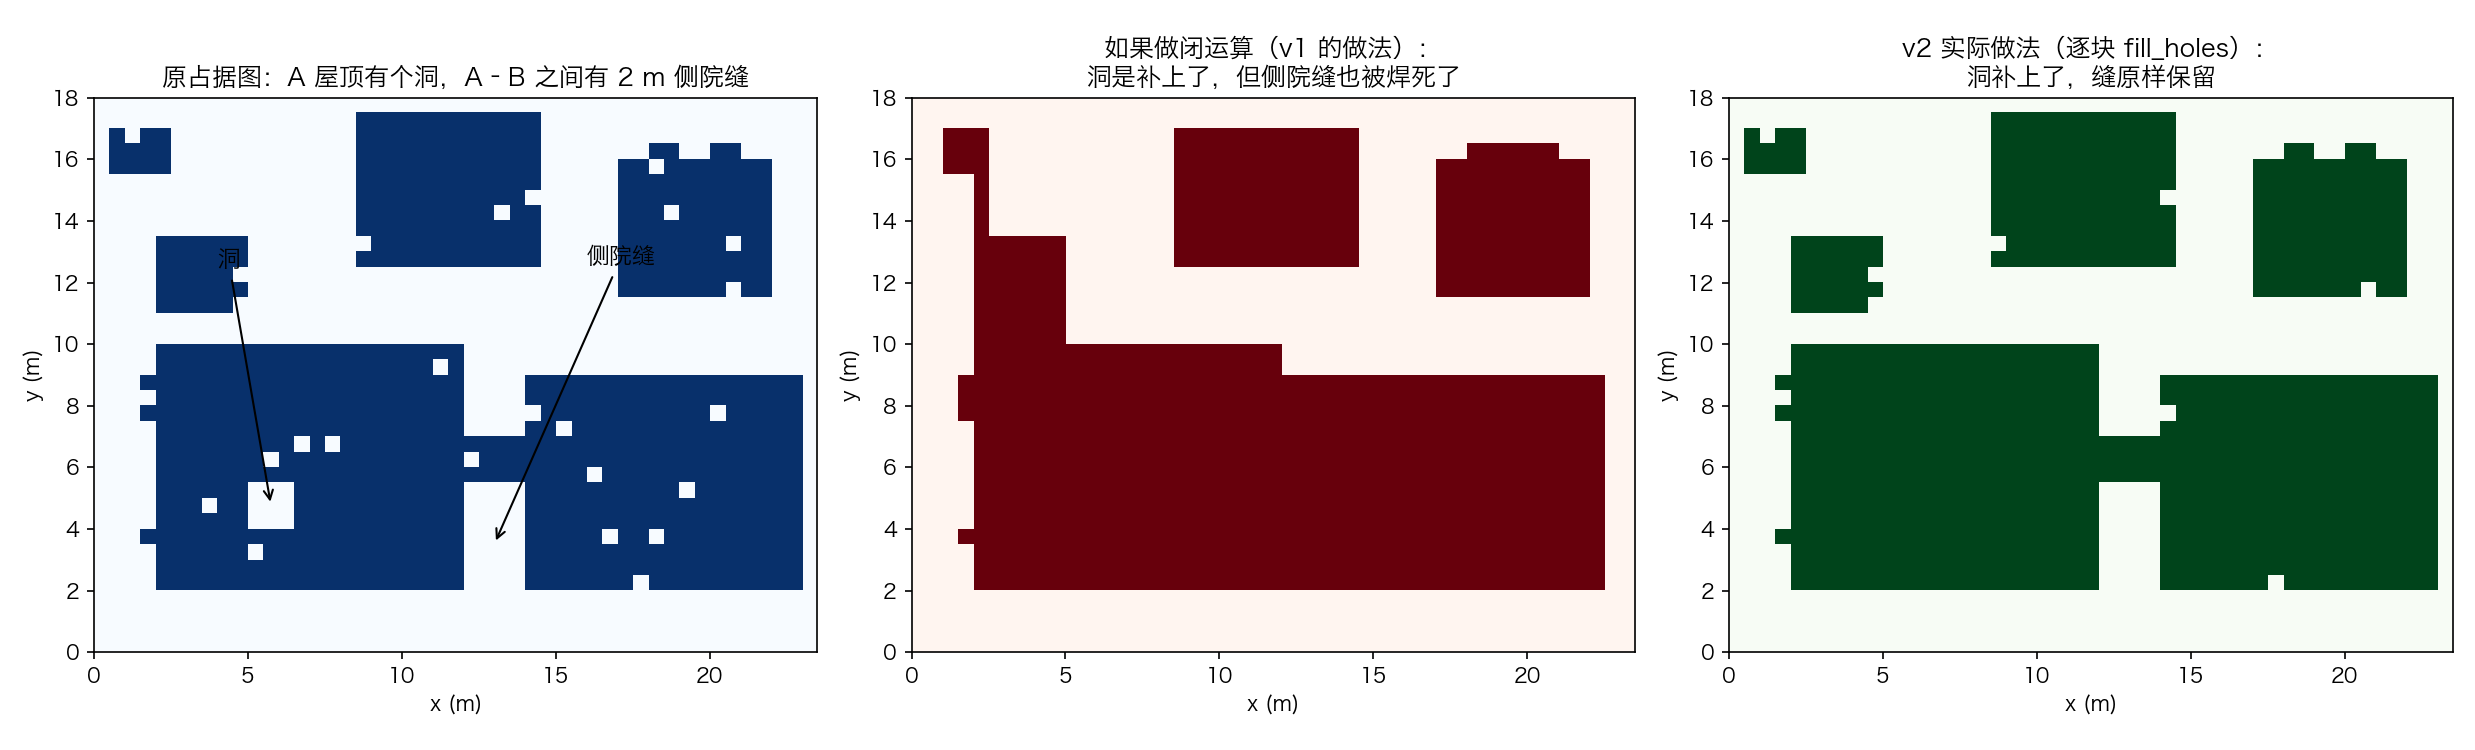
\includegraphics[width=\textwidth]{figs/toy_f4_closing.png}
\caption{第 5 站的两种选择：原图（左）；闭运算的下场（中）；
v2 逐块补洞得到的临时掩膜 \texttt{mf}（右，交给第 6、7 站用）。
中图闭运算的桥接力度和 v1 相当，约 2 米。}
\label{fig:closing}
\end{figure}

\section{第 6 站（123--139 行）：腐蚀取核——查出一块里藏着几栋楼}

\begin{lstlisting}[firstnumber=123]
    selem = disk(int(round(ERODE_R / CELL)))   # 半径 1.5 m 的圆盘
    ...
        core = ndimage.binary_erosion(mf, structure=selem) & m
        lab_c, k = ndimage.label(core, structure=s8)
        if k >= 2:
            sizes = np.bincount(lab_c.ravel())
            valid = [j for j in range(1, k + 1) if sizes[j] >= min_core_cells]
\end{lstlisting}

\begin{whybox}
\texttt{binary\_erosion} 把每个块的边界整整齐齐向里削掉 1.5 米。
这么做的道理很直观：一栋正常的楼宽 8 米往上，削一圈之后中间还剩一大块，
剩下的这部分就叫``核''；要是两栋楼只靠一条\textbf{不到 3 米宽}的``细脖子''连着，
两边各削 1.5 米，脖子必断，剩下两个分开的核。
削完数一数核：有两个以上合格的核（面积至少 6 平方米，免得把屋檐毛刺也当核），
说明这块里不止一栋楼，送下一站拆；只剩一个核、甚至一个不剩的，原样保留。
\end{whybox}

\begin{toybox}
图~\ref{fig:cores}：大块削完剩下\textbf{两个核}，一个是 A 的、一个是 B 的
——1.5 米宽的树桥被削断了。程序到这一步才头一回``发现''大块里藏着两栋楼。
停车场和 C 各剩一个核，门廊、杂物削完什么都不剩：这些块都不拆，原样过站。
\end{toybox}

\begin{figure}[H]
\centering
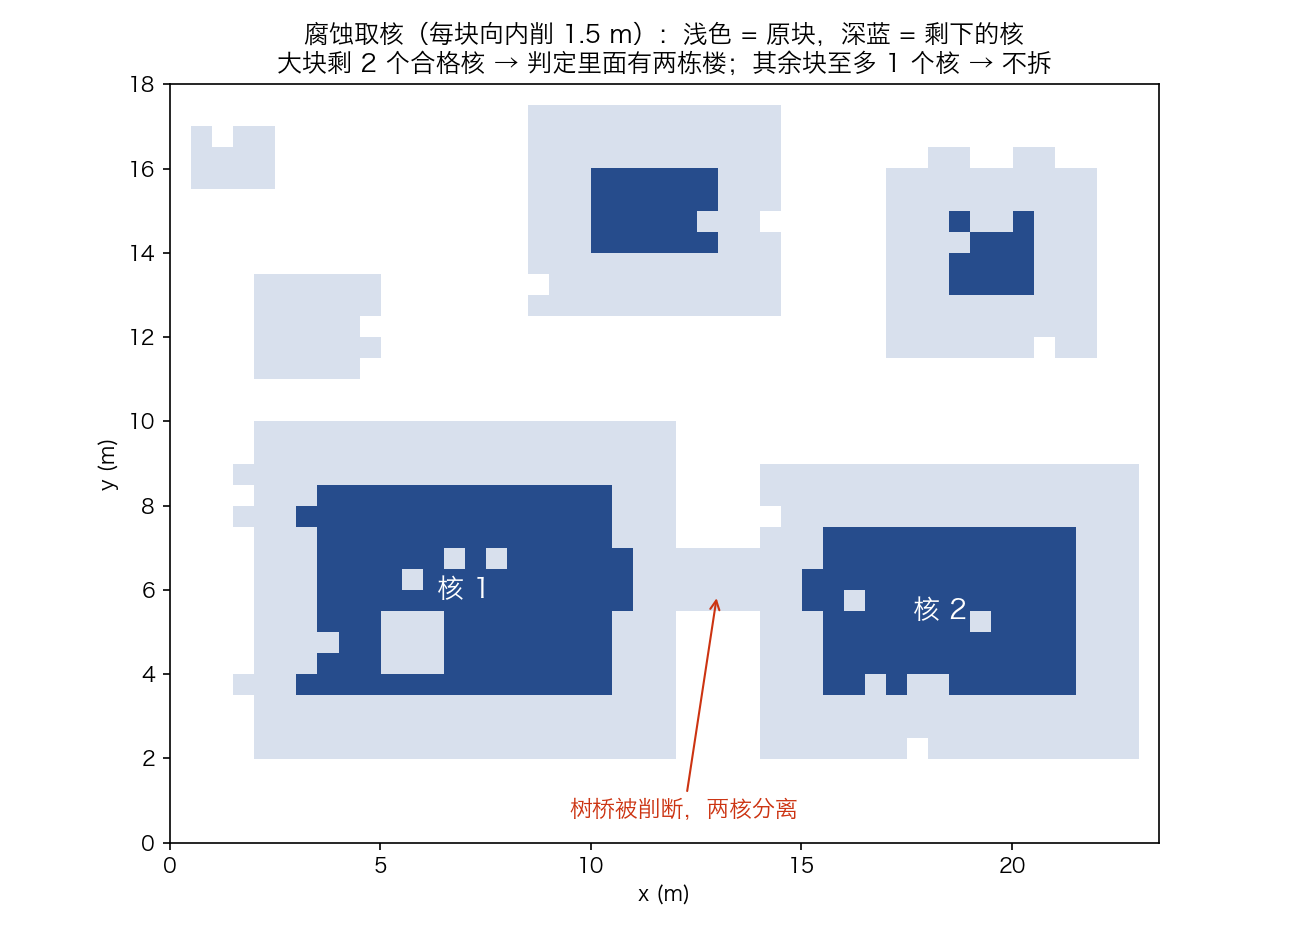
\includegraphics[width=0.72\textwidth]{figs/toy_f5_cores.png}
\caption{第 6 站，腐蚀取核。只有大块削出了两个核，被判定``里面有两栋''。}
\label{fig:cores}
\end{figure}

\section{第 7 站（140--157 行）：marker 分水岭——刀落在高度低谷上}

\begin{lstlisting}[firstnumber=140]
        if len(valid) >= 2:
            markers = np.zeros(m.shape, np.int32)
            for r, j in enumerate(valid, 1):
                markers[lab_c == j] = r            # 每个核 = 一个水源
            ws = watershed(-zg[sl], markers=markers, mask=mf, connectivity=2)
\end{lstlisting}

\begin{whybox}
知道了大块里有两栋楼，刀该落在哪？答案在第 3 站存的高度图 \texttt{zg} 里：
两栋楼的屋顶高，接缝那里——树枝、灌木、地面——低。
沿着``从 A 走到 B''的路线看高度，中间必然经过一段低谷，分界线就该顺着低谷走。

\texttt{watershed}（分水岭）干的正是这件事。它把一张图当成地形往里灌水：
水从指定的水源涨起来（水源就是上一站的核），两片水碰头的地方筑一道坝，
坝就是分割边界。代码里传的是 \texttt{-zg}，高度取了个负号，这是个小技巧：
分水岭天生往洼地里灌水、在高处筑坝，可我们要的坝在低谷。
把高度上下一翻，屋顶就成了盆地，正好当水源；楼间低谷翻成了山脊，
坝自然就筑在了那条线上。\texttt{mask=mf} 则把水拦在本块之内，别处不归它管。
\end{whybox}

\begin{toybox}
看图~\ref{fig:ws}。左图里树桥在高度图上是一道明显的\textbf{暗色低谷}；
中图是分水岭切完的样子，大块顺着树桥被切成了 A、B 两块；
右图沿 $y\approx6.2$ 抽出一行画高度曲线：6 米的 A 顶、2.8 米的低谷、4 米的 B 顶，
红虚线是程序实际切出的边界，正好落在低谷里。
这一站过后，玩具小区从 5 个块变成 \textbf{6 个临时标签}。
真实数据在这一站拆了 \textbf{168 个}多核块，一共拆出 383 份。
\end{toybox}

\begin{figure}[H]
\centering
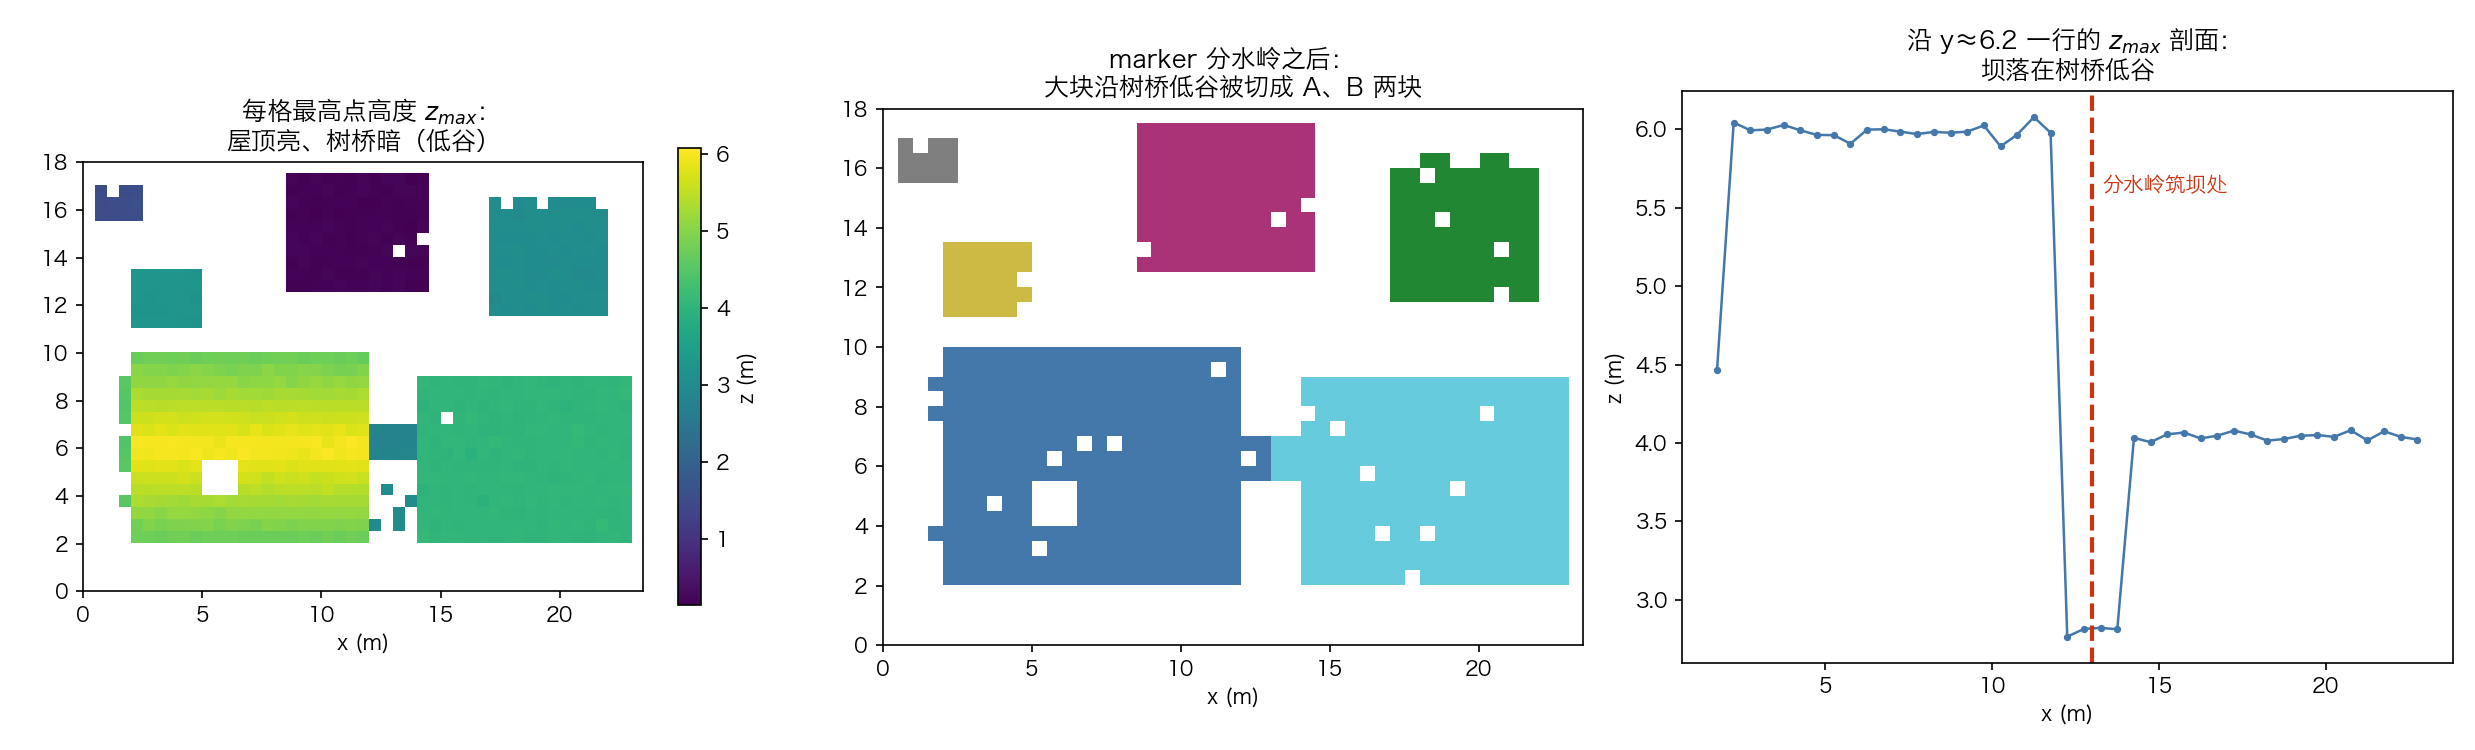
\includegraphics[width=\textwidth]{figs/toy_f6_watershed.png}
\caption{第 7 站：高度图（左）、分水岭拆完（中）、抽一行画剖面验证（右）。}
\label{fig:ws}
\end{figure}

\section{第 8 站（167--208 行）：碎片吸收——只许小的并进大的}

\begin{lstlisting}[firstnumber=193]
    for c in small_ids:                    # 面积 < 20 m2 的碎片
        ...
        d, idx = tree.query(pts, k=1)      # 找最近的"大锚"格子
        j = int(np.argmin(d))
        if d[j] <= ABSORB_DIST + CELL:     # 名义 3 m + 半格补偿
            targ = int(big_l[idx[j]])
            if abs(z50[c] - z50[targ]) <= ABSORB_MAX_DZ:   # 高差 <= 3 m
                remap[c] = targ            # 碎片改姓,并入锚
\end{lstlisting}

\begin{whybox}
不做闭运算，又对粘连块动了刀，偶尔就会矫枉过正：门廊、被树挡剩的小角，
会孤零零变成小碎块，一栋楼碎成``一大一小两个实例''。兜底的规则是：
\textbf{面积不到 20 平方米的碎片，只要 3 米之内有一个 50 平方米以上的``锚''实例，
两边的中位高程又差不到 3 米，就并进锚里}。

三个条件各把一道关。面积门槛管的是\textbf{只许小的并进大的}：
两栋各 50 平方米的真房子，谁也吞不掉谁，吸收机制自己绝不会制造新的粘连。
距离条件保证碎片确实就贴在锚边上——名义上是 3 米，
代码里写的却是 \texttt{ABSORB\_DIST + CELL}：距离按格子的代表点来量，
得多让出半格（0.5 米）的宽容，所以实际判的是 3.5 米以内。
高差条件拦住``隔着高差硬并''的错误，
比如把 10 米高的树冠碎片塞进 4 米高的平房。
\end{whybox}

\begin{toybox}
图~\ref{fig:final} 左：门廊（7.5 平方米）离 A 只有 1.5 米、高差 2.07 米，
三个条件全过，\textbf{并入 A}（红箭头）。杂物团也小，
可它 3 米之内一个大锚都没有，没人收留，先晾着，下一站处理。
棚屋 C 有 23 平方米，压根不算``碎片''，稳稳当当坐在原地。
\end{toybox}

\section{第 9 站（211--228 行）：收尾——丢渣、发号、捡孤儿}

\begin{lstlisting}[firstnumber=211]
    keep = np.nonzero(area2 >= NOISE_AREA)[0]        # < 20 m2 者出局
    ...
    final_id[keep] = np.arange(1, len(keep) + 1, ...)  # 按面积从大到小发号
    inst = final_id[lab_p]
    # 孤儿点: 被 >=2 规则放下的点, 挂回 1.5 m 内最近的实例格
    dist, (ny_i, nx_i) = ndimage.distance_transform_edt(
        final_grid == 0, return_indices=True, sampling=CELL)
    ...
    olab[od > ORPHAN_PT_DIST] = 0
    inst[orphan] = olab
\end{lstlisting}

\begin{whybox}
收尾要做三件事。
第一，\textbf{丢渣}：吸收完还孤零零、面积又不到 20 平方米的小块，按噪声丢掉
——比一间车库还小的独立结构本来就不在建模范围内，错点凑成的假团块也多半是这个尺寸。
第二，\textbf{发号}：幸存的块按面积从大到小，编成正式的 1 号、2 号、3 号\ldots{}。
第三，\textbf{捡孤儿}：第 3 站有一批点，因为所在格子不够 2 个点被暂时放下了，
其中不少其实是真屋顶的边缘。现在把它们挂回 1.5 米之内最近的实例格
（\texttt{distance\_transform\_edt} 一口气算出每个空格到最近实例格的距离和方向）；
1.5 米之内没有实例的，保持无主。
最后（281--295 行）把每个点分到的编号，作为 \texttt{instance\_id} 属性写回点云文件。
交货。
\end{whybox}

\begin{toybox}
图~\ref{fig:final} 右是终局。杂物团（2.8 平方米）被丢掉；
剩下 \textbf{4 个实例}按面积领号：1 号是 A（85 平方米，门廊已并入）、
2 号 B（62）、3 号停车场（29）、4 号 C（22）。
A 左边屋檐的 12 个稀疏点（橙圈）成功挂回了 1 号。
再交代一下第 3 站放下的那批点最后去了哪（实测结果）：
5 个零星错点因为贴着 A、B 的墙边，就近挂靠——2 个归了 1 号、3 个归了 2 号。
桥没搭成，点本身留下来也无伤大雅；杂物团的 72 个点离谁都超过 1.5 米，
没人认领，保持无主。
最后注意：\textbf{3 号停车场还活着}。这个脚本只看``平面上的块''，
对贴着地面的错标毫无办法——所以才需要 Gate A，下一节就讲。
\end{toybox}

\begin{figure}[H]
\centering
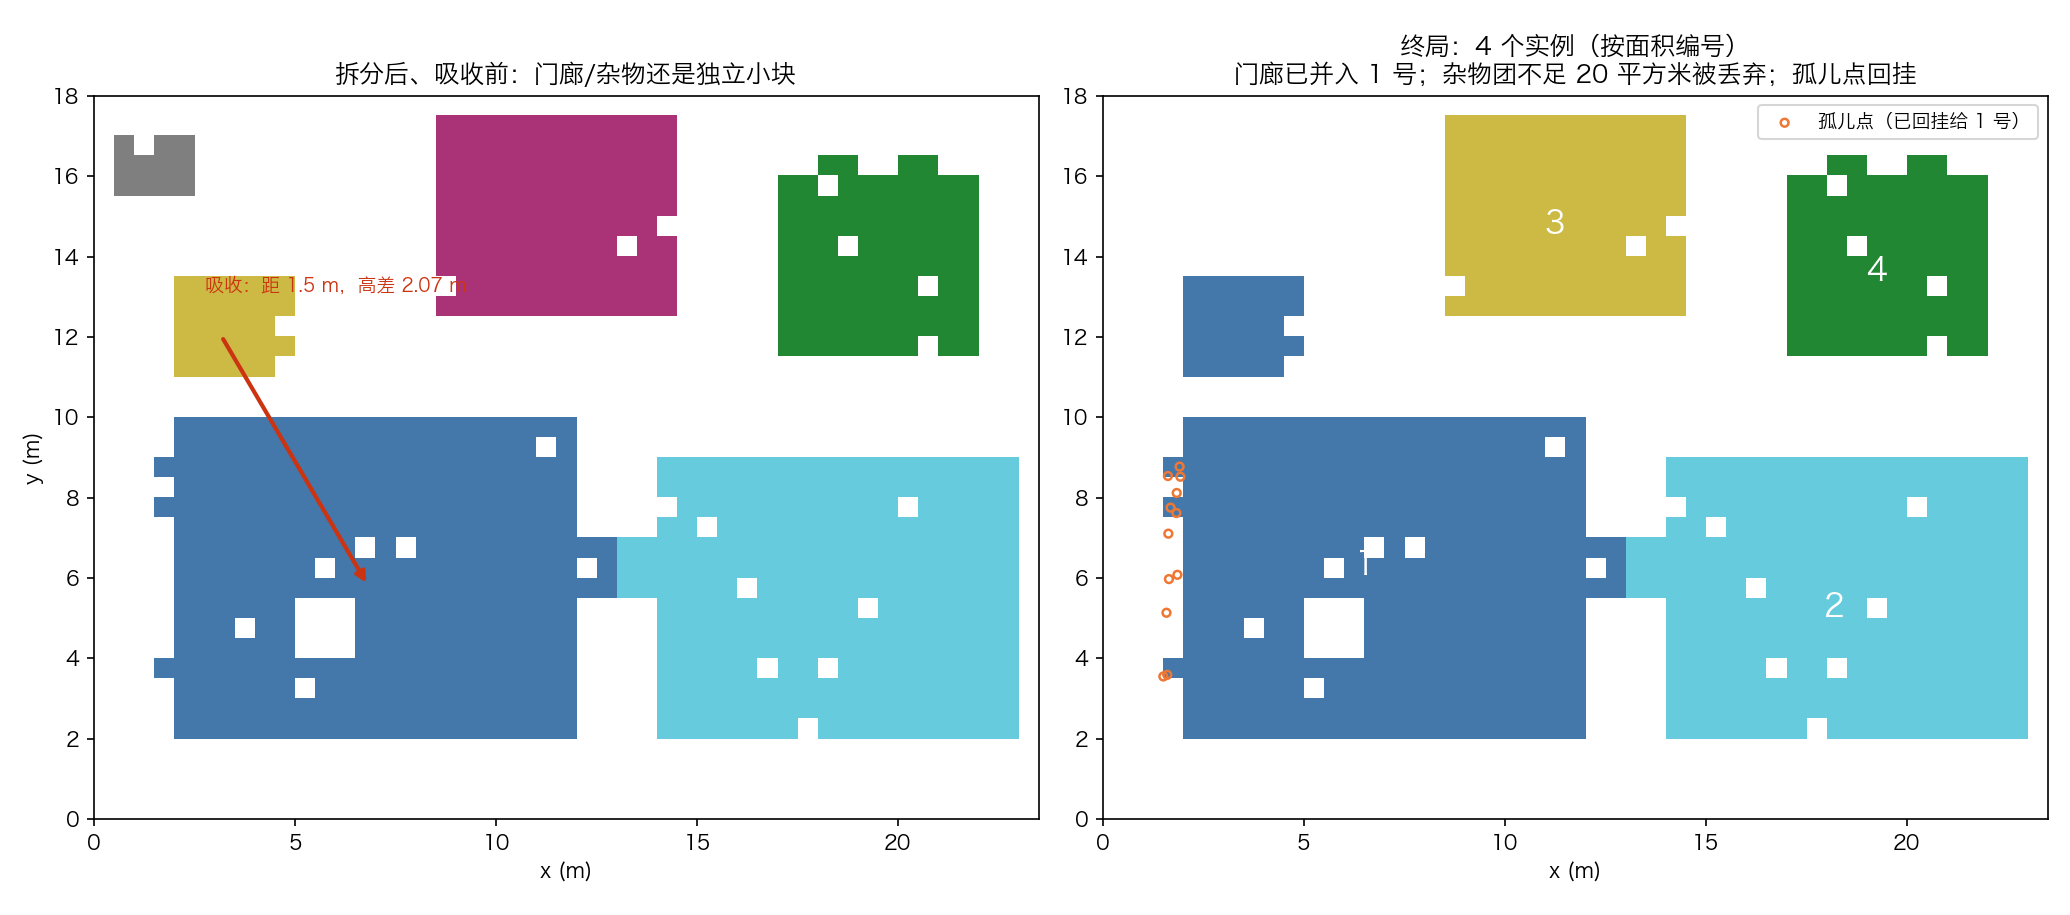
\includegraphics[width=\textwidth]{figs/toy_f7_final.png}
\caption{第 8、9 站前后：先吸收（左，红箭头），再丢渣、发号、捡孤儿（右）。}
\label{fig:final}
\end{figure}

\section{附加站（另一个文件 \texttt{gate\_a\_filter.py}）：算离地高度，请走停车场}

实例分好了，还得把``根本不是楼''的实例请出去。这活儿在另一个脚本
\texttt{gate\_a\_filter.py} 里，核心也就两段代码：

\begin{lstlisting}[firstnumber=73]
dtm = np.full((ny_d, nx_d), np.inf, np.float32)
...
    np.minimum.at(dtm, (gy..., gx...), gz)     # 每格取地面点最低值
dtm_med = ndimage.median_filter(...)           # 去孤立坑/尖
dtm_filled = dtm[iy_n, ix_n]                   # 楼底空缺由最近邻借补
\end{lstlisting}

\begin{lstlisting}[firstnumber=127]
    ring = ndimage.binary_dilation(m, structure=ring_se) & ~m  # 楼周 4 m 环
    ...
    ground = float(np.percentile(src, 5))      # 环内地面高程的第 5 百分位
    hag = z50 - ground                         # 离地高度
    if hag < HAG_MIN:                          # < 2 m: 不可能是楼
        dec = 1
\end{lstlisting}

\begin{whybox}
思路分两步。第一步，用\textbf{类别 2 的地面点}建一张 1 米一格的
\textbf{地面高程图（DTM）}：每格取最低值，中值滤波去掉孤立的坑和尖，
楼底下没有地面回波的空格，就近从旁边``借''一个值补上。
第二步，给每个实例算\textbf{离地高度 HAG}：拿实例的中位高程，
减去楼周围 4 米环带里地面高程的第 5 百分位。
为什么取环带、不取楼底？楼底的值是借来的，环带里才是实测。
为什么取第 5 百分位、不取最小值？防的是个别坏点，图个稳健。
算出来 \textbf{HAG 不到 2 米的，不可能是楼}，剔除。
真实数据里这条规则一次都没触发（真正干掉那 13 个假建筑的，
是细长度和形状两条``机器捞候选、人来拍板''的通道，第一册模块 5 有完整交代），
不过在玩具小区里，它正好有活儿干。
\end{whybox}

\begin{toybox}
图~\ref{fig:gatea}。左边是用地面点建出来的 DTM，楼底下一块块空白，
就是没有地面回波的地方。右边是四个实例的离地高度：
1 号 5.22 米、2 号 3.79 米、4 号 2.74 米，都过线；
\textbf{3 号停车场只有 0.08 米}，撞在 2 米的门槛上，剔除。
玩具小区到此收官：\textbf{3 栋干净建筑}。
\end{toybox}

\begin{figure}[H]
\centering
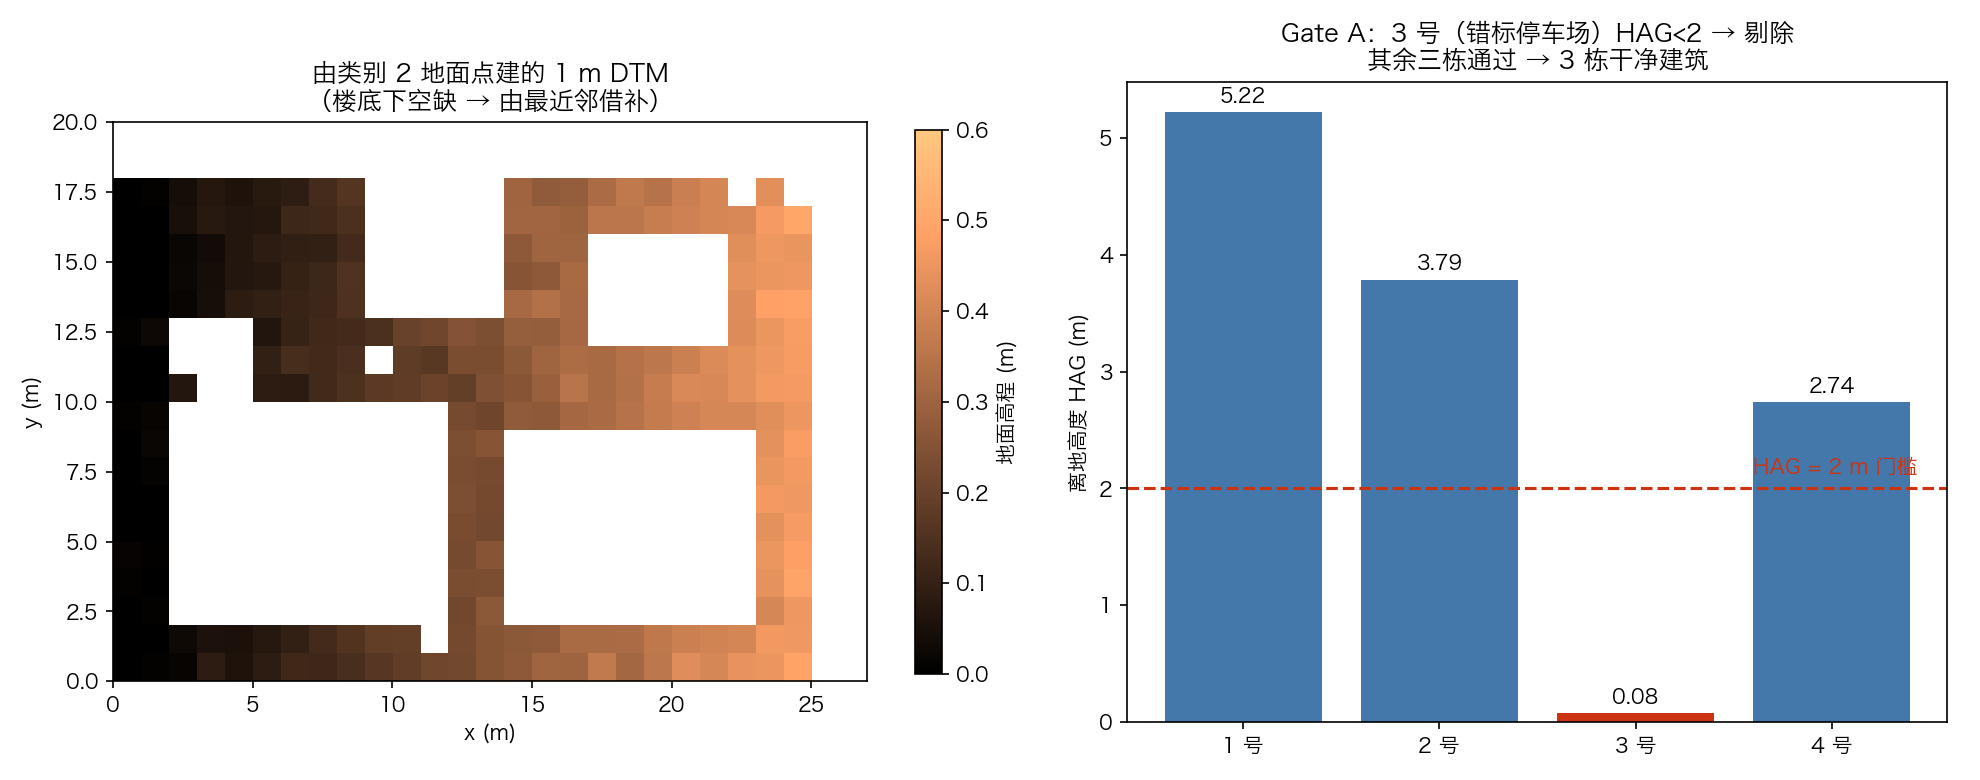
\includegraphics[width=\textwidth]{figs/toy_f8_gatea.png}
\caption{附加站（Gate A 的核心）：DTM（左）和逐实例的离地高度（右）。}
\label{fig:gatea}
\end{figure}

\section{玩具和真实：同一套代码的两份成绩单}

\begin{center}
\small
\begin{tabular}{lll}
\toprule
站点 & 玩具小区（本册实跑） & 真实数据（2.76 km\textsuperscript{2}） \\
\midrule
1 挑建筑点 & 4{,}964 点 & 约 863 万点（占全部点的 11.3\%） \\
3 栅格化 & 809 个占据格；34 个单点格放下 & 0.5 m 格网，数百万格 \\
4 连通域 & 5 块（A、树桥、B 粘成 1 块） & 数千块 \\
6--7 取核、分水岭 & 拆 1 块，得 2 栋 & 拆 \textbf{168} 块，得 383 份（净增 215） \\
8 碎片吸收 & 门廊并入 A（距 1.5 m，高差 2.07 m） & 若干；只许小并大 \\
9 丢渣、发号、孤儿 & 丢杂物 2.8 m\textsuperscript{2}；4 个实例；回挂 34 点 & \textbf{2{,}296 个实例} \\
Gate A（另一文件） & 停车场 HAG 0.08 m 剔除，剩 3 栋 & HAG 规则 0 触发；人工判读剔 13 \\
更下游的追溯修正 & （玩具里没这段剧情） & 剔 22 个树冠、6 栋拆成 12，最终 \textbf{2{,}267 栋} \\
\bottomrule
\end{tabular}
\end{center}

两点提醒。其一，真实数据里 HAG 规则一个都没触发：像玩具停车场那样的目标，
在真实区里根本活不到实例这一步，13 个剔除全部出自细长度和形状规则捞候选、
再人工判读。其二，剔树冠、拆连体楼这两件事发生在更下游，
证据要等第 4 步平面提取和轮廓处理跑完才拿得到，第一册讲义的模块 5、6 讲得很全。

\section{两册讲义怎么配合看}

读代码卡住了，回第一册补概念；读概念觉得空，来本册看实跑。对应关系如下：

\begin{center}
\small
\begin{tabular}{lll}
\toprule
本册 & 内容 & 第一册对应 \\
\midrule
第 1--2 站 & 挑点、换单位 & 模块 1（任务与起点） \\
第 3 站 & 栅格化、``够 2 点才占据'' & 模块 3 前半 \\
第 4--5 站 & 连通域；补洞和闭运算之争 & 模块 3 后半（v1 事故） \\
第 6--7 站 & 取核、分水岭 & 模块 4 \\
第 8--9 站 & 吸收、丢渣、发号、捡孤儿 & 模块 4 后半 \\
附加站 & DTM 和离地高度 & 模块 5 \\
（本册未展开） & 人工判读通道、追溯修正、总台账 & 模块 5--6 \\
（本册未展开） & 参考了哪些论文、路线怎么选的 & 模块 2 \\
\bottomrule
\end{tabular}
\end{center}

\bigskip
\noindent\textbf{想自己重跑}：本册所有玩具图出自同目录的 \texttt{toy\_pipeline.py}，
命令行运行 \texttt{python3 toy\_pipeline.py} 即可。它复刻了
\texttt{instance\_segmentation\_v2.py} 和 \texttt{gate\_a\_filter.py} 的核心操作，
参数和真实管线完全一致：0.5 m 格、每格 2 点、1.5 m 腐蚀、6 m\textsuperscript{2} 核、
20 / 50 m\textsuperscript{2} 面积线、3 m 吸收距离、3 m 高差、1.5 m 回挂、
4 m 环带、第 5 百分位、2 m 离地门槛。

\end{document}
